\documentclass{standalone}
\usepackage{tikz}
\usetikzlibrary{patterns, positioning}

\begin{document}
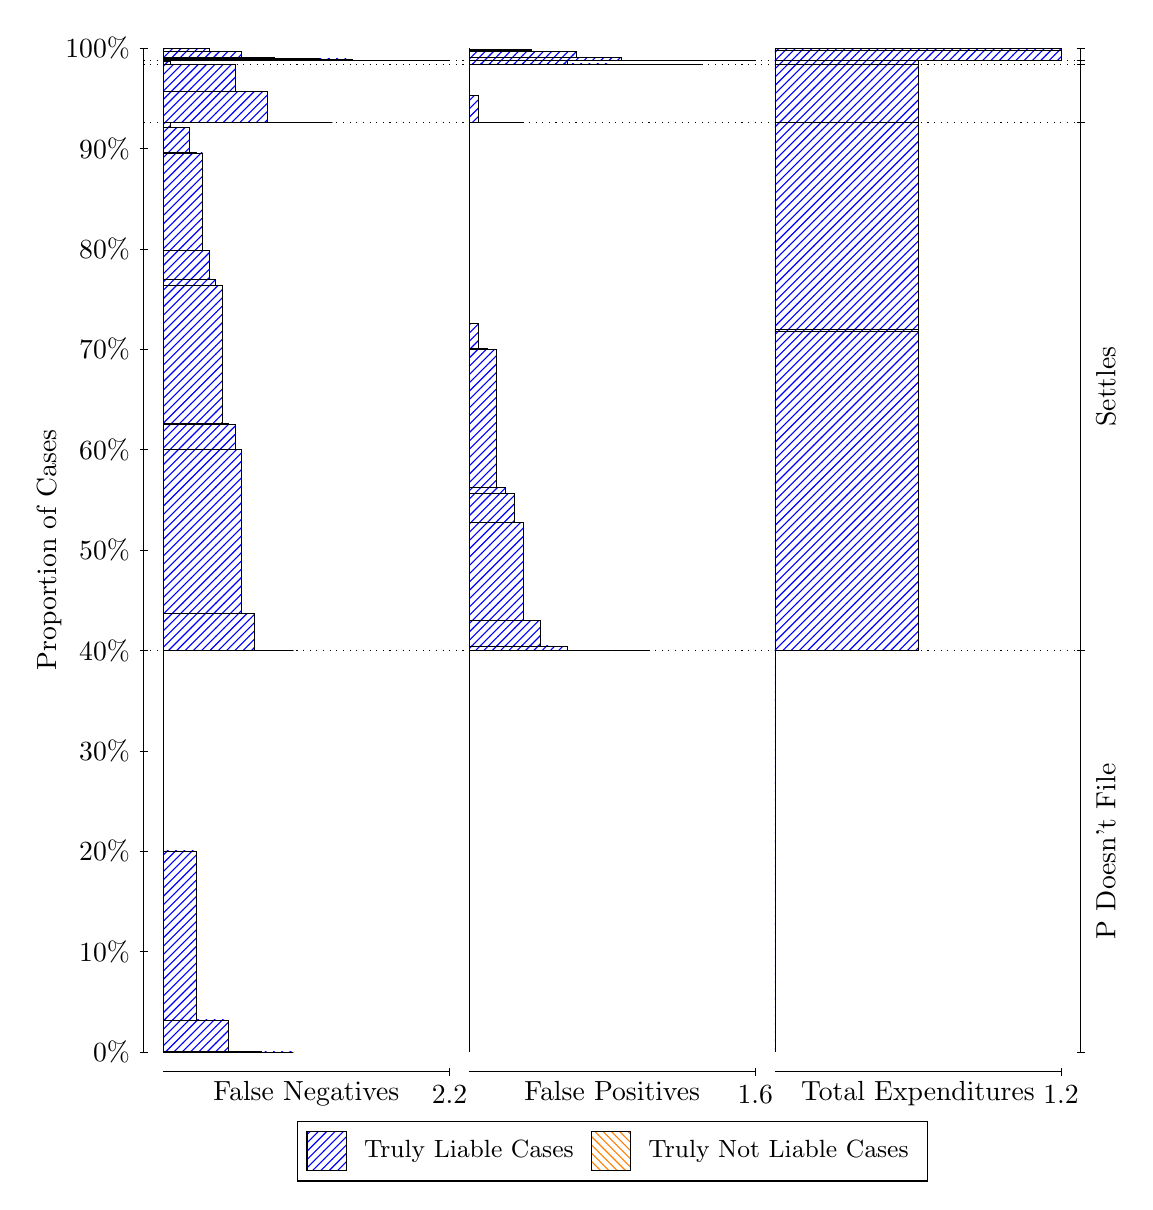
\begin{tikzpicture}
\draw[black, very thin] (1.5,1.75) -- (1.5,14.5);
\node[rotate=90, anchor=center] at (0.3, 8.125) {Proportion of Cases};
\draw[black, very thin] (1.45,1.75) -- (1.55,1.75);
\node[anchor=east] at (1.45, 1.75) {0\%};
\draw[black, very thin] (1.45,3.025) -- (1.55,3.025);
\node[anchor=east] at (1.45, 3.025) {10\%};
\draw[black, very thin] (1.45,4.3) -- (1.55,4.3);
\node[anchor=east] at (1.45, 4.3) {20\%};
\draw[black, very thin] (1.45,5.575) -- (1.55,5.575);
\node[anchor=east] at (1.45, 5.575) {30\%};
\draw[black, very thin] (1.45,6.85) -- (1.55,6.85);
\node[anchor=east] at (1.45, 6.85) {40\%};
\draw[black, very thin] (1.45,8.125) -- (1.55,8.125);
\node[anchor=east] at (1.45, 8.125) {50\%};
\draw[black, very thin] (1.45,9.4) -- (1.55,9.4);
\node[anchor=east] at (1.45, 9.4) {60\%};
\draw[black, very thin] (1.45,10.675) -- (1.55,10.675);
\node[anchor=east] at (1.45, 10.675) {70\%};
\draw[black, very thin] (1.45,11.95) -- (1.55,11.95);
\node[anchor=east] at (1.45, 11.95) {80\%};
\draw[black, very thin] (1.45,13.225) -- (1.55,13.225);
\node[anchor=east] at (1.45, 13.225) {90\%};
\draw[black, very thin] (1.45,14.5) -- (1.55,14.5);
\node[anchor=east] at (1.45, 14.5) {100\%};

\draw[black, very thin] (13.4,1.75) -- (13.4,14.5);
\draw[black, very thin] (13.35,1.75) -- (13.45,1.75);
\node[anchor=west] at (13.35, 1.75) {};
\draw[black, very thin] (13.35,6.8489) -- (13.45,6.8489);
\node[anchor=west] at (13.35, 6.8489) {};
\draw[black, very thin] (13.35,13.552) -- (13.45,13.552);
\node[anchor=west] at (13.35, 13.552) {};
\draw[black, very thin] (13.35,14.294) -- (13.45,14.294);
\node[anchor=west] at (13.35, 14.294) {};
\draw[black, very thin] (13.35,14.342) -- (13.45,14.342);
\node[anchor=west] at (13.35, 14.342) {};
\draw[black, very thin] (13.35,14.5) -- (13.45,14.5);
\node[anchor=west] at (13.35, 14.5) {};

\draw[black, very thin, pattern color=blue, pattern=north east lines] (1.75,1.75) rectangle (3.4015,1.75);
\draw[black, very thin, pattern color=blue, pattern=north east lines] (1.75,1.75) rectangle (2.9886,1.7534);
\draw[black, very thin, pattern color=blue, pattern=north east lines] (1.75,1.7534) rectangle (2.5758,2.158);
\draw[black, very thin, pattern color=blue, pattern=north east lines] (1.75,2.158) rectangle (2.1629,4.3029);
\draw[black, very thin, pattern color=orange, pattern=north west lines] (1.75,4.3029) rectangle (1.75,4.3029);
\draw[black, very thin, pattern color=blue, pattern=north east lines] (1.75,4.3029) rectangle (1.75,6.8489);
\draw[black, very thin, pattern color=blue, pattern=north east lines] (1.75,6.8489) rectangle (3.4015,6.8489);
\draw[black, very thin, pattern color=blue, pattern=north east lines] (1.75,6.8489) rectangle (3.2364,6.8489);
\draw[black, very thin, pattern color=blue, pattern=north east lines] (1.75,6.8489) rectangle (3.0712,6.8498);
\draw[black, very thin, pattern color=blue, pattern=north east lines] (1.75,6.8498) rectangle (2.9886,6.8503);
\draw[black, very thin, pattern color=blue, pattern=north east lines] (1.75,6.8503) rectangle (2.9061,7.3207);
\draw[black, very thin, pattern color=blue, pattern=north east lines] (1.75,7.3207) rectangle (2.8235,7.3248);
\draw[black, very thin, pattern color=blue, pattern=north east lines] (1.75,7.3248) rectangle (2.7409,9.3999);
\draw[black, very thin, pattern color=blue, pattern=north east lines] (1.75,9.3999) rectangle (2.6583,9.7166);
\draw[black, very thin, pattern color=blue, pattern=north east lines] (1.75,9.7166) rectangle (2.5758,9.7317);
\draw[black, very thin, pattern color=blue, pattern=north east lines] (1.75,9.7317) rectangle (2.4932,11.482);
\draw[black, very thin, pattern color=blue, pattern=north east lines] (1.75,11.482) rectangle (2.4106,11.559);
\draw[black, very thin, pattern color=blue, pattern=north east lines] (1.75,11.559) rectangle (2.328,11.926);
\draw[black, very thin, pattern color=blue, pattern=north east lines] (1.75,11.926) rectangle (2.2455,13.168);
\draw[black, very thin, pattern color=blue, pattern=north east lines] (1.75,13.168) rectangle (2.1629,13.174);
\draw[black, very thin, pattern color=blue, pattern=north east lines] (1.75,13.174) rectangle (2.0803,13.493);
\draw[black, very thin, pattern color=blue, pattern=north east lines] (1.75,13.493) rectangle (1.9977,13.497);
\draw[black, very thin, pattern color=blue, pattern=north east lines] (1.75,13.497) rectangle (1.9152,13.499);
\draw[black, very thin, pattern color=blue, pattern=north east lines] (1.75,13.499) rectangle (1.8326,13.552);
\draw[black, very thin, pattern color=orange, pattern=north west lines] (1.75,13.552) rectangle (1.75,13.552);
\draw[black, very thin, pattern color=blue, pattern=north east lines] (1.75,13.552) rectangle (1.75,13.552);
\draw[black, very thin, pattern color=blue, pattern=north east lines] (1.75,13.552) rectangle (3.897,13.552);
\draw[black, very thin, pattern color=blue, pattern=north east lines] (1.75,13.552) rectangle (3.4841,13.56);
\draw[black, very thin, pattern color=blue, pattern=north east lines] (1.75,13.56) rectangle (3.0712,13.952);
\draw[black, very thin, pattern color=blue, pattern=north east lines] (1.75,13.952) rectangle (2.6583,14.29);
\draw[black, very thin, pattern color=blue, pattern=north east lines] (1.75,14.29) rectangle (2.2455,14.294);
\draw[black, very thin, pattern color=orange, pattern=north west lines] (1.75,14.294) rectangle (1.75,14.294);
\draw[black, very thin, pattern color=blue, pattern=north east lines] (1.75,14.294) rectangle (2.2455,14.296);
\draw[black, very thin, pattern color=blue, pattern=north east lines] (1.75,14.296) rectangle (1.8326,14.338);
\draw[black, very thin, pattern color=orange, pattern=north west lines] (1.75,14.338) rectangle (1.75,14.338);
\draw[black, very thin, pattern color=blue, pattern=north east lines] (1.75,14.338) rectangle (1.75,14.342);
\draw[black, very thin, pattern color=blue, pattern=north east lines] (1.75,14.342) rectangle (5.3833,14.342);
\draw[black, very thin, pattern color=blue, pattern=north east lines] (1.75,14.342) rectangle (4.9705,14.342);
\draw[black, very thin, pattern color=blue, pattern=north east lines] (1.75,14.342) rectangle (4.5576,14.346);
\draw[black, very thin, pattern color=blue, pattern=north east lines] (1.75,14.346) rectangle (4.1447,14.363);
\draw[black, very thin, pattern color=blue, pattern=north east lines] (1.75,14.363) rectangle (3.9795,14.363);
\draw[black, very thin, pattern color=blue, pattern=north east lines] (1.75,14.363) rectangle (3.7318,14.364);
\draw[black, very thin, pattern color=blue, pattern=north east lines] (1.75,14.364) rectangle (3.5667,14.364);
\draw[black, very thin, pattern color=blue, pattern=north east lines] (1.75,14.364) rectangle (3.3189,14.364);
\draw[black, very thin, pattern color=blue, pattern=north east lines] (1.75,14.364) rectangle (3.1538,14.384);
\draw[black, very thin, pattern color=blue, pattern=north east lines] (1.75,14.384) rectangle (2.9061,14.384);
\draw[black, very thin, pattern color=blue, pattern=north east lines] (1.75,14.384) rectangle (2.7409,14.462);
\draw[black, very thin, pattern color=blue, pattern=north east lines] (1.75,14.462) rectangle (2.328,14.498);
\draw[black, very thin, pattern color=blue, pattern=north east lines] (1.75,14.498) rectangle (1.9152,14.5);
\draw[black, very thin, pattern color=orange, pattern=north west lines] (1.75,14.5) rectangle (1.75,14.5);
\draw[black, very thin, pattern color=blue, pattern=north east lines] (1.75,14.5) rectangle (1.75,14.5);
\draw[black, very thin, pattern color=orange, pattern=north west lines] (5.6333,1.75) rectangle (5.6333,1.75);
\draw[black, very thin, pattern color=blue, pattern=north east lines] (5.6333,1.75) rectangle (5.6333,6.8489);
\draw[black, very thin, pattern color=orange, pattern=north west lines] (5.6333,6.8489) rectangle (7.9042,6.8489);
\draw[black, very thin, pattern color=blue, pattern=north east lines] (5.6333,6.8489) rectangle (7.9042,6.8489);
\draw[black, very thin, pattern color=orange, pattern=north west lines] (5.6333,6.8489) rectangle (7.6771,6.8489);
\draw[black, very thin, pattern color=blue, pattern=north east lines] (5.6333,6.8489) rectangle (7.6771,6.8489);
\draw[black, very thin, pattern color=orange, pattern=north west lines] (5.6333,6.8489) rectangle (7.45,6.8489);
\draw[black, very thin, pattern color=blue, pattern=north east lines] (5.6333,6.8489) rectangle (7.45,6.8489);
\draw[black, very thin, pattern color=blue, pattern=north east lines] (5.6333,6.8489) rectangle (7.3365,6.8489);
\draw[black, very thin, pattern color=orange, pattern=north west lines] (5.6333,6.8489) rectangle (7.2229,6.8489);
\draw[black, very thin, pattern color=blue, pattern=north east lines] (5.6333,6.8489) rectangle (7.2229,6.8489);
\draw[black, very thin, pattern color=blue, pattern=north east lines] (5.6333,6.8489) rectangle (7.1094,6.8494);
\draw[black, very thin, pattern color=orange, pattern=north west lines] (5.6333,6.8494) rectangle (6.9958,6.8494);
\draw[black, very thin, pattern color=blue, pattern=north east lines] (5.6333,6.8494) rectangle (6.9958,6.8494);
\draw[black, very thin, pattern color=blue, pattern=north east lines] (5.6333,6.8494) rectangle (6.8823,6.9022);
\draw[black, very thin, pattern color=blue, pattern=north east lines] (5.6333,6.9022) rectangle (6.7687,6.904);
\draw[black, very thin, pattern color=blue, pattern=north east lines] (5.6333,6.904) rectangle (6.6552,6.9081);
\draw[black, very thin, pattern color=blue, pattern=north east lines] (5.6333,6.9081) rectangle (6.5417,7.2267);
\draw[black, very thin, pattern color=blue, pattern=north east lines] (5.6333,7.2267) rectangle (6.4281,7.233);
\draw[black, very thin, pattern color=blue, pattern=north east lines] (5.6333,7.233) rectangle (6.3146,8.4753);
\draw[black, very thin, pattern color=blue, pattern=north east lines] (5.6333,8.4753) rectangle (6.201,8.8422);
\draw[black, very thin, pattern color=blue, pattern=north east lines] (5.6333,8.8422) rectangle (6.0875,8.9188);
\draw[black, very thin, pattern color=blue, pattern=north east lines] (5.6333,8.9188) rectangle (5.974,10.669);
\draw[black, very thin, pattern color=blue, pattern=north east lines] (5.6333,10.669) rectangle (5.8604,10.685);
\draw[black, very thin, pattern color=blue, pattern=north east lines] (5.6333,10.685) rectangle (5.7469,11.001);
\draw[black, very thin, pattern color=blue, pattern=north east lines] (5.6333,11.001) rectangle (5.6333,13.552);
\draw[black, very thin, pattern color=orange, pattern=north west lines] (5.6333,13.552) rectangle (6.3146,13.552);
\draw[black, very thin, pattern color=blue, pattern=north east lines] (5.6333,13.552) rectangle (6.3146,13.556);
\draw[black, very thin, pattern color=blue, pattern=north east lines] (5.6333,13.556) rectangle (5.7469,13.895);
\draw[black, very thin, pattern color=blue, pattern=north east lines] (5.6333,13.895) rectangle (5.6333,14.294);
\draw[black, very thin, pattern color=orange, pattern=north west lines] (5.6333,14.294) rectangle (8.5854,14.294);
\draw[black, very thin, pattern color=blue, pattern=north east lines] (5.6333,14.294) rectangle (8.5854,14.294);
\draw[black, very thin, pattern color=blue, pattern=north east lines] (5.6333,14.294) rectangle (8.0177,14.294);
\draw[black, very thin, pattern color=blue, pattern=north east lines] (5.6333,14.294) rectangle (7.45,14.299);
\draw[black, very thin, pattern color=blue, pattern=north east lines] (5.6333,14.299) rectangle (6.8823,14.34);
\draw[black, very thin, pattern color=blue, pattern=north east lines] (5.6333,14.34) rectangle (6.3146,14.342);
\draw[black, very thin, pattern color=orange, pattern=north west lines] (5.6333,14.342) rectangle (9.2667,14.342);
\draw[black, very thin, pattern color=blue, pattern=north east lines] (5.6333,14.342) rectangle (9.2667,14.342);
\draw[black, very thin, pattern color=orange, pattern=north west lines] (5.6333,14.342) rectangle (8.699,14.342);
\draw[black, very thin, pattern color=blue, pattern=north east lines] (5.6333,14.342) rectangle (8.699,14.342);
\draw[black, very thin, pattern color=orange, pattern=north west lines] (5.6333,14.342) rectangle (8.1313,14.342);
\draw[black, very thin, pattern color=blue, pattern=north east lines] (5.6333,14.342) rectangle (8.1313,14.345);
\draw[black, very thin, pattern color=blue, pattern=north east lines] (5.6333,14.345) rectangle (7.5635,14.381);
\draw[black, very thin, pattern color=orange, pattern=north west lines] (5.6333,14.381) rectangle (7.5635,14.381);
\draw[black, very thin, pattern color=blue, pattern=north east lines] (5.6333,14.381) rectangle (7.5635,14.381);
\draw[black, very thin, pattern color=blue, pattern=north east lines] (5.6333,14.381) rectangle (6.9958,14.457);
\draw[black, very thin, pattern color=blue, pattern=north east lines] (5.6333,14.457) rectangle (6.9958,14.458);
\draw[black, very thin, pattern color=orange, pattern=north west lines] (5.6333,14.458) rectangle (6.7687,14.458);
\draw[black, very thin, pattern color=blue, pattern=north east lines] (5.6333,14.458) rectangle (6.7687,14.458);
\draw[black, very thin, pattern color=blue, pattern=north east lines] (5.6333,14.458) rectangle (6.4281,14.468);
\draw[black, very thin, pattern color=blue, pattern=north east lines] (5.6333,14.468) rectangle (6.4281,14.478);
\draw[black, very thin, pattern color=orange, pattern=north west lines] (5.6333,14.478) rectangle (6.201,14.478);
\draw[black, very thin, pattern color=blue, pattern=north east lines] (5.6333,14.478) rectangle (6.201,14.478);
\draw[black, very thin, pattern color=blue, pattern=north east lines] (5.6333,14.478) rectangle (5.8604,14.478);
\draw[black, very thin, pattern color=blue, pattern=north east lines] (5.6333,14.478) rectangle (5.8604,14.478);
\draw[black, very thin, pattern color=orange, pattern=north west lines] (5.6333,14.478) rectangle (5.6333,14.478);
\draw[black, very thin, pattern color=blue, pattern=north east lines] (5.6333,14.478) rectangle (5.6333,14.5);
\draw[black, very thin, pattern color=orange, pattern=north west lines] (9.5167,1.75) rectangle (9.5167,1.75);
\draw[black, very thin, pattern color=blue, pattern=north east lines] (9.5167,1.75) rectangle (9.5167,6.8489);
\draw[black, very thin, pattern color=orange, pattern=north west lines] (9.5167,6.8489) rectangle (11.333,6.8489);
\draw[black, very thin, pattern color=blue, pattern=north east lines] (9.5167,6.8489) rectangle (11.333,10.906);
\draw[black, very thin, pattern color=orange, pattern=north west lines] (9.5167,10.906) rectangle (11.333,10.906);
\draw[black, very thin, pattern color=blue, pattern=north east lines] (9.5167,10.906) rectangle (11.333,10.927);
\draw[black, very thin, pattern color=orange, pattern=north west lines] (9.5167,10.927) rectangle (11.333,10.927);
\draw[black, very thin, pattern color=blue, pattern=north east lines] (9.5167,10.927) rectangle (11.333,13.552);
\draw[black, very thin, pattern color=orange, pattern=north west lines] (9.5167,13.552) rectangle (11.333,13.552);
\draw[black, very thin, pattern color=blue, pattern=north east lines] (9.5167,13.552) rectangle (11.333,14.294);
\draw[black, very thin, pattern color=orange, pattern=north west lines] (9.5167,14.294) rectangle (11.333,14.294);
\draw[black, very thin, pattern color=blue, pattern=north east lines] (9.5167,14.294) rectangle (11.333,14.342);
\draw[black, very thin, pattern color=orange, pattern=north west lines] (9.5167,14.342) rectangle (13.15,14.342);
\draw[black, very thin, pattern color=blue, pattern=north east lines] (9.5167,14.342) rectangle (13.15,14.467);
\draw[black, very thin, pattern color=orange, pattern=north west lines] (9.5167,14.467) rectangle (13.15,14.467);
\draw[black, very thin, pattern color=blue, pattern=north east lines] (9.5167,14.467) rectangle (13.15,14.5);
\draw[black, dotted] (1.5,6.8489) -- (13.4,6.8489);
\draw[black, dotted] (1.5,13.552) -- (13.4,13.552);
\draw[black, dotted] (1.5,14.294) -- (13.4,14.294);
\draw[black, dotted] (1.5,14.342) -- (13.4,14.342);
\draw[black, very thin] (1.75,1.5) -- (5.3833,1.5);
\node[anchor=north] at (3.5667, 1.5) {False Negatives};
\draw[black, very thin] (5.3833,1.45) -- (5.3833,1.55);
\node[anchor=north] at (5.3833, 1.45) {2.2};

\draw[black, very thin] (5.6333,1.5) -- (9.2667,1.5);
\node[anchor=north] at (7.45, 1.5) {False Positives};
\draw[black, very thin] (9.2667,1.45) -- (9.2667,1.55);
\node[anchor=north] at (9.2667, 1.45) {1.6};

\draw[black, very thin] (9.5167,1.5) -- (13.15,1.5);
\node[anchor=north] at (11.333, 1.5) {Total Expenditures};
\draw[black, very thin] (13.15,1.45) -- (13.15,1.55);
\node[anchor=north] at (13.15, 1.45) {1.2};

\node[black, centered, rotate=90] at (13.72, 4.2994) {P Doesn't File};
\node[black, centered, rotate=90] at (13.72, 10.201) {Settles};




\draw (7.449999999999999,1.5) node[draw=none] (baseCoordinate) {};
\begin{scope}[align=center]
        \matrix[scale=0.5, draw=black, below=0.5cm of baseCoordinate, nodes={draw}, column sep=0.1cm]{
            \node[rectangle, draw, minimum width=0.5cm, minimum height=0.5cm, pattern=north east lines, pattern color=blue] {}; &
            \node[draw=none, font=\small] (B) {Truly Liable Cases}; &
            \node[rectangle, draw, minimum width=0.5cm, minimum height=0.5cm, pattern=north west lines, pattern color=orange] {}; &
            \node[draw=none, font=\small] (B) {Truly Not Liable Cases}; \\
            };
\end{scope}

\end{tikzpicture}
\end{document}